\documentclass[a4paper,11pt]{article}
\usepackage[utf8]{inputenc}
\usepackage[T1]{fontenc}
\usepackage{amsmath}
\usepackage{mathtools}
\usepackage{amsfonts}
\usepackage{amssymb}
\usepackage{graphicx}
\usepackage{multicol}
\usepackage{array}
\usepackage{float}
\usepackage{epstopdf}
\usepackage{caption}
\usepackage{subcaption}
\usepackage{gensymb}
\usepackage[bottom]{footmisc}
\usepackage{appendix}
\usepackage{pdfpages}
\usepackage{todonotes}
\usepackage{mathpazo}
\usepackage{titleps}
\usepackage{color}
\usepackage{xcolor}
\usepackage{colortbl}
\usepackage{siunitx}
\usepackage{pdflscape}
\usepackage{cancel}

\usepackage[skins]{tcolorbox}
\usepackage{sectsty}
\usepackage[arrowmos]{circuitikz}
\usepackage{pgfplots}
\usepackage{blindtext}
\usepackage[inner=2cm,outer=2cm,top=2.5cm,bottom=2.5cm]{geometry}
\usepackage{todonotes}
\usepackage{hyperref}
\usepackage{url}
\usepackage{adjustbox}
\usepackage{tabularx}
\usepackage{booktabs}
\usepackage{fancybox}
\usepackage[tikz]{bclogo}



%For code insertion
%listing
\usepackage{listings}
\usepackage{xcolor}
\definecolor{codegreen}{rgb}{0,0.6,0}
\definecolor{codegray}{rgb}{0.5,0.5,0.5}
\definecolor{codepurple}{rgb}{0.58,0,0.82}
\definecolor{backcolour}{rgb}{0.98,0.98,0.98}
\lstdefinestyle{mystyle}{
    backgroundcolor=\color{backcolour},
    commentstyle=\color{codegreen},
    keywordstyle=\color{blue},
    numberstyle=\tiny\color{codegray},
    stringstyle=\color{codepurple},
    basicstyle=\ttfamily\footnotesize,
    breakatwhitespace=false,
    breaklines=true,
    captionpos=b,
    keepspaces=true,
    numbers=left,
    numbersep=5pt,
    showspaces=false,
    showstringspaces=false,
    showtabs=false,
    tabsize=2
}
\lstset{style=mystyle}



\graphicspath{{figures/}}
\sectionfont{\large}
\subsectionfont{\normalsize}
%%%%%%%%%%%%%%%%%%%
% HANDS-ON NUMBER
\newcommand\handsOnN{FIR}
% WEEK NUMBER
\newcommand\weekN{9}
%%%%%%%%%%%%%%%%%%%

\newpagestyle{main}{
	\sethead[LELEC2103][][]{LELEC2103}{}{}
	\headrule
    \setfoot[][\thepage][]{}{\thepage}{}
}

\newcommand{\horrule}[1]{\rule{\linewidth}{#1}} % Create horizontal rule command with 1 argument of height
%%%%%%%%%%%%%%%%%%%%%%%%%%%%%%%%%%%%%%%%%%%%%%%%%%%%%%%%%%%%%%%%%%%%%%%%%%%%

\begin{document}
\renewcommand{\figurename}{Fig.}

\renewcommand{\thepage}{\arabic{page}}
\setcounter{page}{1}
\pagestyle{main}
\newpage \clearpage

\begin{center}
\begin{huge}
LELEC2102: Programming the FIR on the LimeSDR FPGA\\
\end{huge}
\vspace{0.3cm}
%\textit{TA 1, TA 2}
\end{center}

\section*{Introduction}

In this Hands-On, you will be introduced to the basics of microcontroller unit (MCU) operation and interrupt-based embedded programming. We will use so-called bare metal programming, which means we will not use an operating system: you will be in control of all the code that runs on the device! As this is most likely your first project dealing with bare metal embedded programming, we will provide you with a functional baseline code to start with. Then, you will be guided step by step to develop the key skills needed for this part of the project.
\begin{bclogo}[couleur = gray!20, arrondi = 0.2, logo=\bcinfo]{Explanation of the hands-on boxes}
In this note, there are a few boxes presenting additional information:
\begin{itemize}
    \item \bcinfo will provide you some more detailed explanations.
    \item \bcattention will explain typical mistakes that might lead to errors or a non functional system.
    \item \bcquestion will provide you with additional questions or experiments that will improve your understanding of the system. We advise you to leave them for the end of the hands-on as they are not critical.
\end{itemize}
\end{bclogo}


\section{Packet formatting}

The transmitted packets shall have the following format
\begin{center}
\texttt{r$\mathbin\Vert$emitter\_id$\mathbin\Vert$payload\_length$\mathbin\Vert$packet\_serial$\mathbin\Vert$app\_data$\mathbin\Vert$tag}
\end{center}
(\texttt{$\mathbin\Vert$} denotes concatenation)
where
\begin{center}
\begin{tabular}{lccl}
    Field & Length (bytes) & Encoding & Description \\ \hline
    \texttt{r} & 1 & & Reserved, set to 0.\\
    \texttt{emitter\_id} & 1 & BE & Unique id of the sensor node.\\
    \texttt{payload\_length} & 2 & BE & Length of \texttt{app\_data} (in bytes).\\
    \texttt{packet\_serial} & 4 & BE & Unique and incrementing id of the packet. \\
    \texttt{app\_data} & any  &  & The feature vectors. \\
    \texttt{tag} & 16 & & Message authentication code (MAC). \\
\end{tabular}
\end{center}

\begin{bclogo}[couleur = gray!20, arrondi = 0.2, logo=\bcquestion]{Reserved byte}
    What could be the purpose of a ``reserved'' byte ?
\end{bclogo}
\begin{bclogo}[couleur = gray!20, arrondi = 0.2, logo=\bcinfo]{Endiannes}
    As you can see, a packet is defined as a sequence of bytes and is formed by
    the concatenation of multiple fields.
    Some of those fields are integers that are encoded on multiple bytes (since
    encoding e.g. a 32-bit integer on a single byte is not possible) and we
    therefore need to specify the encoding, that is, the mapping between the
    number and the byte sequence.
    For unsigned fixed-size integers, there are two very common byte encoding:
    little endian (LE) and big endian (BE).
    Let us take the example of a 32-bit unsigned integer, that is a number $x \in
    \{0,\dots, 2^{32}-1\}$.
    Let $x_0,x_1,x_2,x_3\in\{0,...,255\}$ be such that $x = \sum_{i=0}^3 x_i 256^i$.
    The LE encoding of $x$ is \texttt{$x_0$$\mathbin\Vert$$x_1$$\mathbin\Vert$$x_2$$\mathbin\Vert$$x_3$} (the least
    significant byte comes first) while its BE encoding is
    \texttt{$x_3$$\mathbin\Vert$$x_2$$\mathbin\Vert$$x_1$$\mathbin\Vert$$x_0$}.  (the most significant byte comes
    first).
    The LE/BE encodings work similarly for encoding 16-bit (resp. 64-bit,
    128-bit\dots) numbers on 2 (resp. 8, 16\dots) bytes.
    For 8-bit numbers encoded on one byte, the BE and LE encodings are identical.
\end{bclogo}

\begin{bclogo}[couleur = gray!20, arrondi = 0.2, logo=\bcinfo]{Features encoding}
    The feature vectors are a list of MEL vectors (ordered by acquisition
    time), and each MEL vector is a list of 16-bit numbers (ordered from lower
    to higher frequency band).
    The \texttt{app\_data} contains sequentially the MEL vectors, and the
    encoding of each MEL vector is the concatenation (respecting the order) of
    the encoding of the numbers it is made of.  The numbers are encoded on
    2~bytes, in BE.
    You do not need to implement this (it is already done in the \verb|encode_packet| function).
\end{bclogo}

As for each hands-on, start by synchronizing your Git. In the MCU code, the function in charge of forming the packet is
\verb|make_packet| in \texttt{packet.c}.
Its prototype is:
\begin{lstlisting}[style=customc]
int make_packet(uint8_t *packet, size_t payload_len, uint8_t sender_id, uint32_t serial);
\end{lstlisting}
This function takes as input \texttt{packet}, a buffer of bytes of length
\texttt{PACKET\_HEADER\_LENGTH + payload\_len + PACKET\_TAG\_LENGTH}, in
which \texttt{app\_data} should already have been written starting at byte\\
\verb|packet[PACKET_HEADER_LENGTH]|.
The function has to write the remaining parts of the packet (the header and the tag) in the buffer and return the total length of the packet.

\textbf{
    Implement \texttt{make\_packet}, except for the \texttt{tag} part of the
    packet, which is already set by an incorrect function that we will work on afterwards.
    Check that your implementation does not trigger any compiler warning, then
    check that the packet are now decoded correctly on your PC. Be aware that the \texttt{app\_data} data field is already included in the packet\footnote{You can take a look at the method \texttt{encode\_packet} in \texttt{adc\_dblbuf.c} to see how it is done.}.
}

\section{Message authentication code}

Let us now consider the authentication of the message. The authentication
\texttt{tag} is defined as
\[
    \texttt{tag} = \text{CBC-MAC-AES}_{k}\left(
        \texttt{r$\mathbin\Vert$emitter\_id$\mathbin\Vert$payload\_length$\mathbin\Vert$packet\_serial$\mathbin\Vert$app\_data}
    \right)\;,
\]
where $k$ is a secret key (an sequence of 16 bytes) shared between the sensor
node and the receiver. This secret key should be uniformly random. The $\text{CBC-MAC-AES}$ algorithm is described in \autoref{algo:cbc-mac-aes} and its block diagram is shown in \autoref{fig:cbc-mac-aes}.

\begin{bclogo}[couleur = gray!20, arrondi = 0.2, logo=\bcquestion]{What does an authentication tag do ?}
    You have had a quick introduction to the authentication basic knowledge in Lecture L3b.\\
    Based on that and on the description of the message authentication code, what is your understanding of the purpose of the authentication tag ? What does it prevent or allow ?\\
    More importantly, what \textit{doesn't} it prevent ? Is the header readable or encrypted ? And the message data ?
\end{bclogo}

\begin{algorithm}
\begin{algorithmic}
    \REQUIRE Message $x$ (sequence of bytes) to authenticate.
    \REQUIRE Secret key $k$ (sequence of 16 bytes)
    \ENSURE The authentication tag $t$ (sequence of 16 bytes).
    \STATE Parse $x$ into blocks $\left(x_1,x_2,\dots,x_n\right)$ such that the
    length of each block is 16 bytes (except for $x_n$).
    \STATE If the length of $x_n$ is not 16, append as many zero bytes to $x_n$
    to extend it to 16 bytes.
    \STATE $s \leftarrow 0^{16}$ (Where $0^{16}$ denotes the string made of 16 zero bytes.)
    \FOR{$i=1\dots,n$}
    \STATE $s \leftarrow \text{AES}_k(s \oplus x_i)$
    \ENDFOR
    \STATE $t \leftarrow s$
\end{algorithmic}
\caption{CBC-MAC-AES}
\label{algo:cbc-mac-aes}
\end{algorithm}

\begin{figure}[h]
\centering
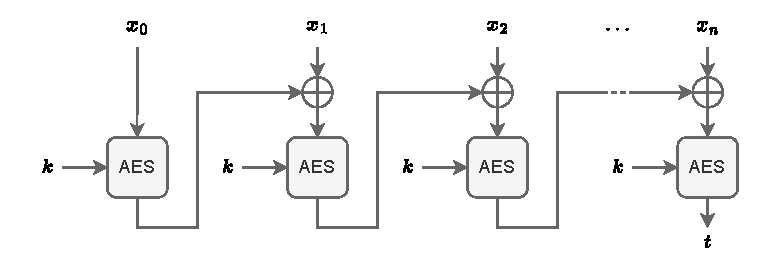
\includegraphics[scale=1]{figures/crypto_cbc_mac_aes.pdf}
\caption{Block diagram of CBC-MAC-AES}
\label{fig:cbc-mac-aes}
\end{figure}

You have to complete the function \texttt{tag\_cbc\_mac()}, which is already present in the \texttt{packet.c} file, by implementing the CBC-MAC-AES algorithm with the following constraints: the function \textbf{must not allocate memory}, and its stack space usage must be constant (i.e., independent of the message length).
We provide you the AES reference implementation (\texttt{aes\_ref.h}), whose
prototype is the following:
\begin{lstlisting}[style=customc]
void AES128_encrypt(unsigned char* block, const unsigned char* key);
\end{lstlisting}
where \texttt{block} is both the input and output of the AES block cipher (it
is modified in-place).
Both \texttt{block} and \texttt{key} are expected to point to 16-byte buffers. Regarding the key, you can modify and use the \texttt{AES\_Key} variable defined on top of the file.

\textbf{
    First, re-write the CBC-MAC-AES algorithm to make it easier to
    implement with the given constraints. Once your have the pseudo-code, translate it in C. Check that your implementation does not trigger any compiler warning.
}

If there are no errors, we are now going to compile and launch the whole MCU application for the project. To do so, go in the \texttt{config.h} file and change the \texttt{RUN\_CONFIG} from \texttt{EVAL\_RADIO} to \texttt{MAIN\_APP}. You can now recompile the design and flash it on the MCU. Launch the GNU Radio \texttt{main\_app} (do not forget to change the carrier frequency). To authenticate the packets, you need to launch a script. To do so, refer to the \texttt{README} of the \texttt{auth} subdirectory.

\section{Performance characterization}
At the end of the semester, you will have to characterize your system. Regarding the MCU, you might want to have an insight on the number of cycle of a given task, as well as the code size. Here are a few tools you can use to extract such information. In order to verify the performance of an implementation, one needs to measure it's key metrics, namely the cycle count, and the code size. We provide you here with explanations on how to make these measurements. Additionally, when compiling, several optimizations steps are provided by the compiler. Those are grouped into optimization levels for ease of use. Follow the explanations in the corresponding box to change the optimization levels.


\begin{bclogo}[couleur = gray!20, arrondi = 0.2, logo=\bcinfo]{How to measure cycle counts} In order to measure the time taken by an implementation, the most basic way is to use a time measuring device, however, this is not precise enough as the MCU can execute several millions of cycles every second. A more accurate method is to measure the number of cycles taken by the CPU. To do so, you will need a special register that is a cycle counter. For ARM processors, if a cycle counter is present, the two registers of interest are :
\begin{lstlisting}[style=customc]
DWT->CTRL |= 1 ; // enable the counter
DWT->CYCCNT = 0; // reset the counter
\end{lstlisting}
After your implementation has run, you can read the value contained in \texttt{DWT->CYCCNT} to read the number of cycles since you set the counter to zero.\\

However, if you try this several times on an implementation whose inputs stay the same, you will probably observe that the numbers change slightly. This is due to interrupts happening during the measured execution. In order to have accurate measurements, you should also disable interrupts during measurement. To do so, use the  \texttt{\_\_disable\_irq()} and \texttt{\_\_enable\_irq()} methods.

Finally, you can take a look at \texttt{utils.c} where wrappers for cycle counting are included that also print the result for easier debugging.
\end{bclogo}



\begin{bclogo}[couleur = gray!20, arrondi = 0.2, logo=\bcinfo]{Choosing the optimization level of the compiler}
	To change the compiler optimization level:
	\begin{enumerate}
		\item Open the project properties : In the top menu-bar, \textbf{Project} $\rightarrow$ \textbf{Properties}.
		\item In the left panel, select \textbf{C/C++ Build} $\rightarrow$ \textbf{Settings}.
		\item Select a build configuration (default choice is Debug or Release, you may also create new ones).
		\item Under the \textbf{Tool Settings} tab, select \textbf{MCU GCC Compiler} $\rightarrow$ \textbf{Optimization}
		\item Select the optimization level.
		\item You may choose the build configuration using the arrow next to the ``Build'' (hammer) icon.
		\item To program the MCU using a chosen build configuration:
		\begin{enumerate}
			\item Use the arrow next to the ``Run'' icon $\rightarrow$ \textbf{Run configurations...}
			\item Create the launch configuration using \textbf{New launch configuration} (icon on the top left)
			\item Change the name of the new configuration (if needed).
			\item Select the binary to program using \textbf{C/C++ Application}
			$\rightarrow$ \textbf{Search project...}, and select the right
			binary (you should have build it before).
		\end{enumerate}
	\end{enumerate}
\end{bclogo}

\begin{bclogo}[couleur = gray!20, arrondi = 0.2, logo=\bcquestion]{Optimization level}
    What are the different optimization levels you can choose ? How do they differ from each other, which metrics do they change ? Which one should you choose for what purpose ?
\end{bclogo}

\begin{bclogo}[couleur = gray!20, arrondi = 0.2, logo=\bcinfo]{How to know the code size}
	A simple way to know the code size of a specific function, such as the AES, is
	to exclude it from the build, rebuild, and compare the total code size
	difference. To do so,
	\begin{enumerate}
		\item Build the complete program using the chosen configuration, and take
		note of the program memory usage (FLASH in the ``Build analyzer''
		window).
		\item Right click on the file you want exclude, \textbf{Resource
			configurations} $\rightarrow$ \textbf{Exclude from build}, for the chosen build configuration.
		\item Fix resulting build errors (you should not call functions that are excluded from build!).
		\item Rebuild and take note of the memory usage.
	\end{enumerate}
\end{bclogo}


\end{document}

%%%%%%%%%%%%%%%%%%%%%%%%%%%%%%%%%%%%%%%%%%%%%%%%%%%%%%%%%%%%%%%%%%%%%%%%%%%%
